\documentclass[a4paper]{jsarticle}

%======================================================================
%		論文のタイトル,著者,日付
%======================================================================

\title{\Huge 知的情報処理論\\\huge 第2回レポート\vspace{120mm}}
\author{\Large 濱崎 直紀\vspace{30mm}}
\date{令和元年6月30日}

%======================================================================
%		マクロの読み込みとコマンドの定義
%======================================================================

\usepackage{graphicx}       % eps file を張り付けるのに必要
\usepackage{amsmath}
%\usepackage[dvipdfmx]{graphicx}     % png等の画像を貼りつけるのに必要
\usepackage{bm}     % 太字を書くのに必要
\usepackage{here}       % その場所に画像を入れるのに必要
\usepackage{comment}        % コメントを挟むのに必要
\usepackage{listings}      % ソースコードを表示するのに必要
\usepackage{jlisting}       % ソースコード内に日本語のコメントアウトがある場合必要(TEX Live の場合,別途ダウンロードが必要)
\newcommand{\argmax}{\mathop{\rm arg~max}\limits}
\newcommand{\argmin}{\mathop{\rm arg~min}\limits}

%======================================================================
%		本文
%======================================================================

\begin{document}

\begin{titlepage}
\maketitle
\thispagestyle{empty}
\end{titlepage}

\section{Work1}
\subsection*{問題}
何らかの識別問題または回帰問題を設定し,それを機械学習により解く.
さらに,評価データとして,学習データをそのまま使用,学習データとは異なるデータを使用,の2つの場合の性能を比較する.

\subsection{概要}
MNISTの0~9の数字が描かれた画像に対して,機械学習によって描かれている数字を分類する分類器を作成し,その精度を測った.
機械学習の手法にはSVM(Support Vector Machine)を用いた.
以下ではその結果と考察を述べる.

\subsection{結果}
分類の精度を以下に示す.
\begin{table}[H]
    \begin{center}
        \begin{tabular}{cc}
            \hline
            Data & Accuracy\\
            \hline \hline
            Training data & 99.0\%\\
            Test data & 97.9\%\\
            \hline
        \end{tabular}
    \end{center}
\end{table}

\subsection{考察}
実際に精度を測る際に、学習データをそのまま用いて測ることをオープンテスト(open test),学習に使わずに用意しておいたテスト用のデータを用いて測ることをクローズドテスト(closed test)と言う.
今回の分類に関しても両者で精度を測り,結果として,オープンテストでは99.0\%,クローズドテストでは97.9\%という結果が得られた.
比較してみると,オープンテストの方がクローズドテストよりもわずかに高い精度が達成された.
学習の際には学習用のデータをうまく分類できるように学習するため,学習用のデータに対しては精度が高く,それと比較して,未知のデータであるテスト用のデータに対しては低くなるのは妥当な結果であると言えるだろう.\par
今回のように,データを学習用とテスト用のデータに分けて,それぞれのデータを用いて学習とテストを行うことを交差検証と言う.
これは,学習用のデータを分類することに適合し過ぎるあまり,未知のデータに対する分類がうまくいかない(過学習)といった問題を防ぐことが期待される.

\section{Work2}
\subsection*{問題}
統計的パターン認識において,確率密度関数$p(\bm{x}|C_i)$が多次元正規分布で表される場合において,以下の(a)から(c)について示す.\par
ここで,多次元正規分布は以下の式で表される.
\begin{equation*}
    p(\bm{x}|C_i)=\frac{1}{(2\pi)^{d/2}\left|\bm{\sum}_i\right|^{1/2}}\exp\left\{-\frac{1}{2}(\bm{x}-m_i)^t{{\bm{\sum}}_i}^{-1}(\bm{x}-m_i)\right\}
\end{equation*}
\begin{enumerate}
    \renewcommand{\labelenumi}{(\alph{enumi})}
    \item 識別関数$g_i(\bm{x})$は$\bm{x}$の2次関数となる.
    \item 共分散行列が全クラスで等しい($\sum_i=\sum_0$)と仮定した場合,識別関数$g_i(\bm{x})$は$\bm{x}$の一次関数,つまり線形識別関数となる.
    \item $\sum_0$を単位行列であるとし,事前確率が各クラスで等しい($P(C_i)=\frac{1}{c}$;$c$はクラス数)とすると,識別関数$g_i(x)$はNearest Neighbour法と同じ形になる.
    この時のクラス$C_i$のプロトタイプがどのように求められるか示す。
\end{enumerate}

\subsection*{解答}
\begin{enumerate}
    \renewcommand{\labelenumi}{(\alph{enumi})}
    \item
    \begin{align*}
        g_i(\bm{x})&=\log{P(\bm{x}|C_i)}+\log{P(C_i)}\\
        &=\log{\frac{1}{(2\pi)^{d/2}\left|\bm{\sum}_i\right|^{1/2}}\exp\left\{-\frac{1}{2}(\bm{x}-m_i)^t{{\bm{\sum}}_i}^{-1}(\bm{x}-m_i)\right\}+\log{P(C_i)}}\\
        &=-\frac{1}{2}\left\{(\bm{x}-m_i)^t{{\bm{\sum}}_i}^{-1}(\bm{x}-m_i)\right\}-\frac{d}{2}\log{2\pi}-\frac{1}{2}\log{\left|{\bm{\sum}}_i\right|}+\log{P(C_i)}
    \end{align*}
    よって,識別関数$g_i(\bm{x})$は$\bm{x}$の2次関数となる.
    \item
    クラス$i,j$に関して考えると,共分散行列が全クラスで等しいことから
    \begin{equation*}
        p(C_i|\bm{x})=p(C_j|\bm{x})
    \end{equation*}
    つまり
    \begin{equation*}
        p(\bm{x}|C_i)p(C_i)=p(\bm{x}|C_j)p(C_j)
    \end{equation*}
    両辺の対数をとって
    \begin{equation}
        \log{p(\bm{x}|C_i)}+\log{p(C_i)}=\log{p(\bm{x}|C_j)}+\log{p(C_j)}
        \label{eq1}
    \end{equation}
    ここで$\lambda_i=\frac{1}{(2\pi)^{d/2}\left|\bm{\sum}_i\right|^{1/2}}$とおくと$p(\bm{x}|C_i)=\lambda_i\exp\left\{-\frac{1}{2}(\bm{x}-m_i)^t{{\bm{\sum}}_i}^{-1}(\bm{x}-m_i)\right\}$となるので
    \begin{align*}
        \log{p(\bm{x}|C_i)}&=\log{\lambda_i}-\frac{1}{2}(\bm{x}-m_i)^t{{\bm{\sum}}_i}^{-1}(\bm{x}-m_i)\\
        &=\log{\lambda_i}-\frac{1}{2}\left\{\bm{x}^t{{\bm{\sum}}_0}^{-1}\bm{x}-2m_i^t{\bm{\sum}}^{-1}\bm{x}+m_i^t{\bm{\sum}}^{-1}m_i\right\}
    \end{align*}
    これを式(\ref{eq1})に代入すると
    \begin{align*}
        \log\lambda_0-\frac{1}{2}\bm{x}^t{{\bm{\sum}}_0}^{-1}\bm{x}+m_i^t{{\bm{\sum}}_0}^{-1}\bm{x}-\frac{1}{2}m_i^t{{\bm{\sum}}_0}^{-1}m_i+\log{P(C_i)}\\
        =\log\lambda_0-\frac{1}{2}\bm{x}^t{{\bm{\sum}}_0}^{-1}\bm{x}+m_j^t{{\bm{\sum}}_0}^{-1}\bm{x}-\frac{1}{2}m_j^t{{\bm{\sum}}_0}^{-1}m_j+\log{P(C_j)}
    \end{align*}
    よって
    \begin{align*}
        g(\bm{x})&=log{P(C_i|\bm{x})}-log{P(C_j|\bm{x})}\\
        &=m_i^t{{\bm{\sum}}_0}^{-1}\bm{x}-m_j^t{{\bm{\sum}}_0}^{-1}\bm{x}-\frac{1}{2}m_i^t{{\bm{\sum}}_0}^{-1}m_i+\log{P(C_i)}+\frac{1}{2}m_i^t{{\bm{\sum}}_0}^{-1}m_i-\log{P(C_i)}\\
        &=(m_i-m_j)^t{{\bm{\sum}}_0}^{-1}\bm{x}+\left\{-\frac{1}{2}m_i^t{{\bm{\sum}}_0}^{-1}m_i+\log{P(C_i)}+\frac{1}{2}m_i^t{{\bm{\sum}}_0}^{-1}m_i-\log{P(C_i)}\right\}
    \end{align*}
    よって,識別関数$g_i(\bm{x})$は線形識別関数となる.
    \item
    \begin{align*}
        g_i(\bm{x})&=\log{P(C_i|\bm{x})}\\
        &=\log{P(\bm{x}|C_i)}+\log{P(C_i)}\\
        &=\log{P(\bm{x}|C_i)}-\log{c}
    \end{align*}
    ここで,$\sum_0$が単位行列,事前確率が各クラスで等しいということから
    \begin{align*}
        \log{P(\bm{x}|C_i)}&=\log\lambda_i-\frac{1}{2}(\bm{x}-m_i)^t{\bm{\sum}}_i^{-1}(\bm{x}-m_i)\\
        &=\log{\lambda_0}-\frac{1}{2}||\bm{x}-m_i||^2
    \end{align*}
    よって
    \begin{align*}
        g_i(\bm{x})&=\log{P(\bm{x}|C_i)}-\log{c}\\
        &=\log{\lambda_0}-\frac{1}{2}||\bm{x}-m_i||^2-\log{c}\\
        &=-\frac{1}{2}||\bm{x}-m_i||^2+\log{\frac{\lambda_0}{c}}
    \end{align*}
    ゆえに
    \begin{align*}
        \argmax_i{g_i(\bm{x})}&=\argmax_i\left\{-\frac{1}{2}||\bm{x}-m_i||^2+\log{\frac{\lambda_0}{c}}\right\}\\
        &=\argmax_i\left\{-||\bm{x}-m_i||^2\right\}\\
        &=\argmin_i\left\{||\bm{x}-m_i||^2\right\}
    \end{align*}
\end{enumerate}


%======================================================================
%		付録
%======================================================================

\clearpage
\appendix
\pagestyle{empty}
% ソースコードの表示に関する設定
\lstset{
    basicstyle={\ttfamily},
    identifierstyle={\small},
    commentstyle={\smallitshape},
    keywordstyle={\small\bfseries},
    ndkeywordstyle={\small},
    stringstyle={\small\ttfamily},
    frame={tb},
    breaklines=true,
    columns=[l]{fullflexible},
    numbers=left,
    xrightmargin=0zw,
    xleftmargin=3zw,
    numberstyle={\scriptsize},
    stepnumber=1,
    numbersep=1zw,
    lineskip=-0.5ex
}

\setcounter{figure}{1}
\begin{figure}[p]
    \begin{center}
        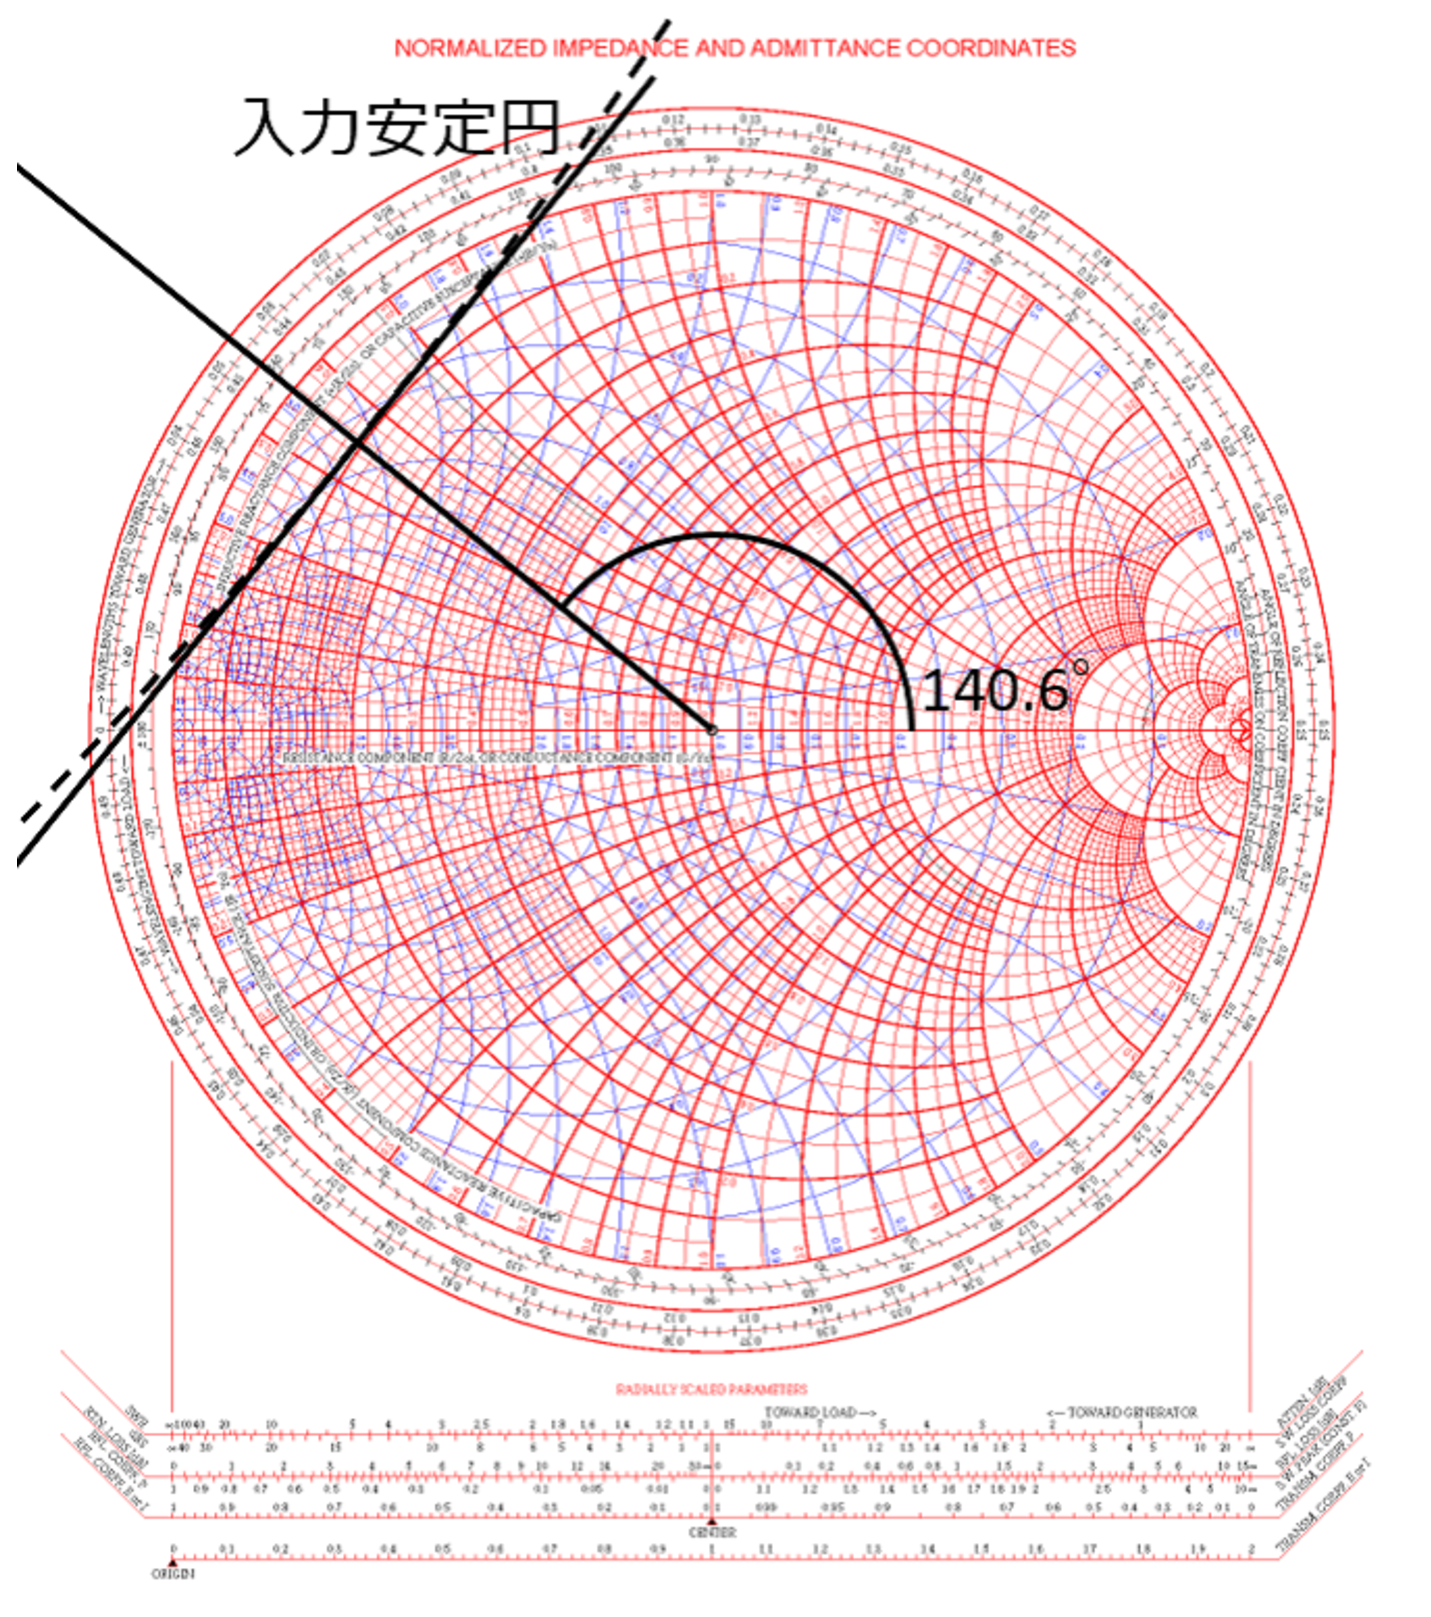
\includegraphics[width=175mm]{./figures/section/2.eps}
        \caption{}
    \end{center}
\end{figure}
\clearpage
\setcounter{figure}{2}
\begin{figure}[p]
    \begin{center}
        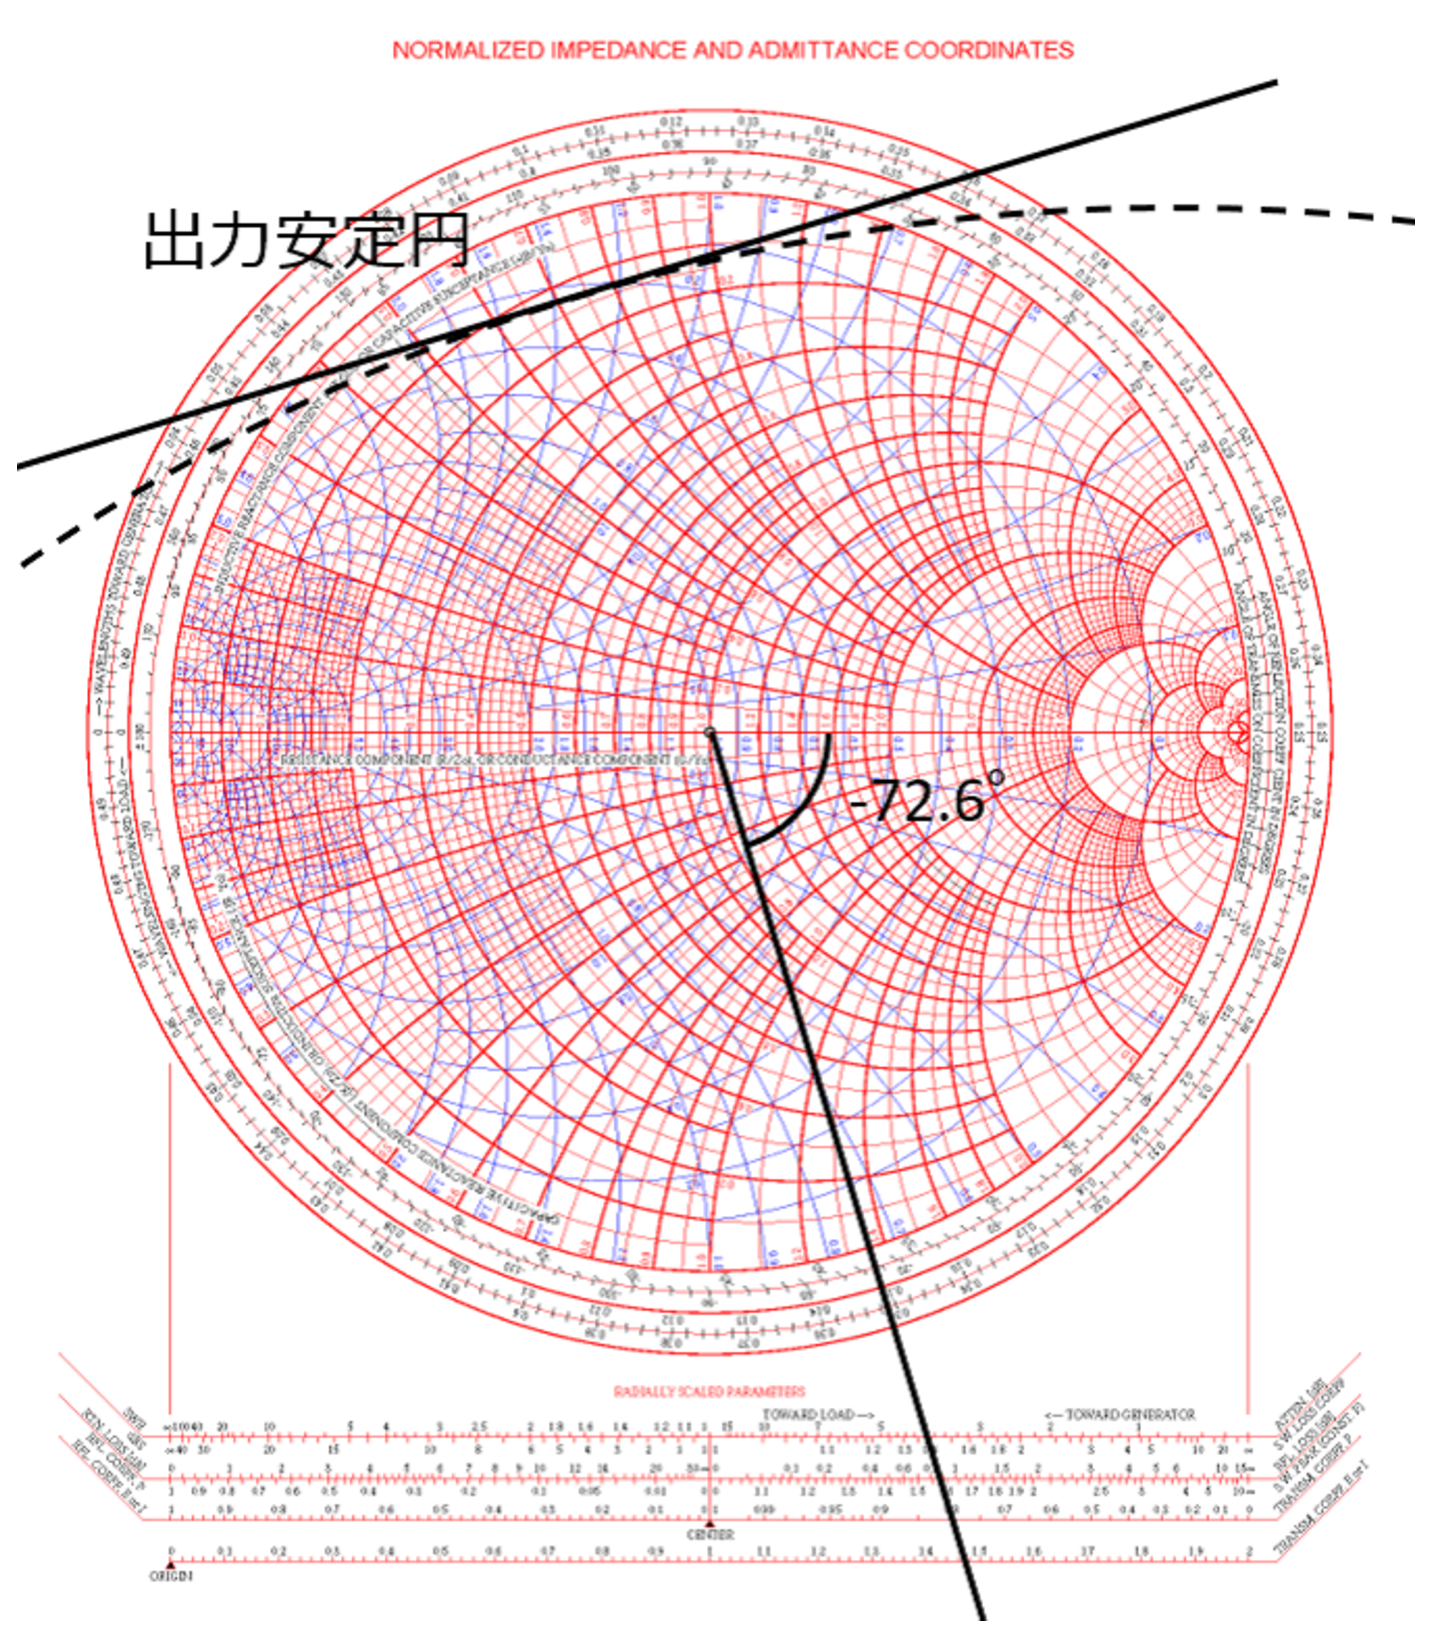
\includegraphics[width=175mm]{./figures/section/3.eps}
        \caption{}
    \end{center}
\end{figure}

\end{document}
